\documentclass[a4paper,11pt]{report}

\usepackage{amsmath,amssymb}
\usepackage{fullpage}
\usepackage{graphicx}

\usepackage{bussproofs}
\usepackage{mathpartir}
\usepackage{prooftrees}
\usepackage{color}
\usepackage{rotating}



\usepackage{tikz}
\usetikzlibrary{automata,positioning}
\usetikzlibrary{fit}

\newcommand*\circled[1]{\tikz[baseline=(char.base)]{
    \node[shape=circle,draw,inner sep=2pt] (char) {#1};}}

\makeatletter
\pgfmathdeclarefunction{alpha}{1}{%
  \pgfmathint@{#1}%
  \edef\pgfmathresult{\pgffor@alpha{\pgfmathresult}}%
}

\newcommand*{\until}{U}
\newcommand*{\disj}{\ ,\ }
\newcommand*{\A}{\square}  % Always
\newcommand*{\D}{\diamondsuit} % eventually

\newcommand*{\Pq}{(\top,\bot)}
\newcommand*{\pQ}{(\bot,\top)}
\newcommand*{\PQ}{(\top,\top)}
\newcommand*{\pq}{(\bot,\bot)}


% tikz
\usepackage{tikz}
\usetikzlibrary{snakes}



\author{Sylvain Julmy}
\date{\today}

\setlength{\parindent}{0pt}
\setlength{\parskip}{2.5pt}

\begin{document}

\begin{center}
  \Large{
    Automata on Infinite Structure\\
    Fall 2018
  }
  
  \noindent\makebox[\linewidth]{\rule{\linewidth}{0.4pt}}
  Exercice Sheet 7

  \vspace*{1.4cm}

  Author : Sylvain Julmy
  \noindent\makebox[\linewidth]{\rule{\linewidth}{0.4pt}}

  \begin{flushleft}
    Professor : Ultes-Nitsche Ulrich
    
    Assistant : Stammet Christophe
  \end{flushleft}

  \noindent\makebox[\linewidth]{\rule{\textwidth}{1pt}}
\end{center}

\section*{Exercise 1}

{\centering
  \begin{turn}{90}
    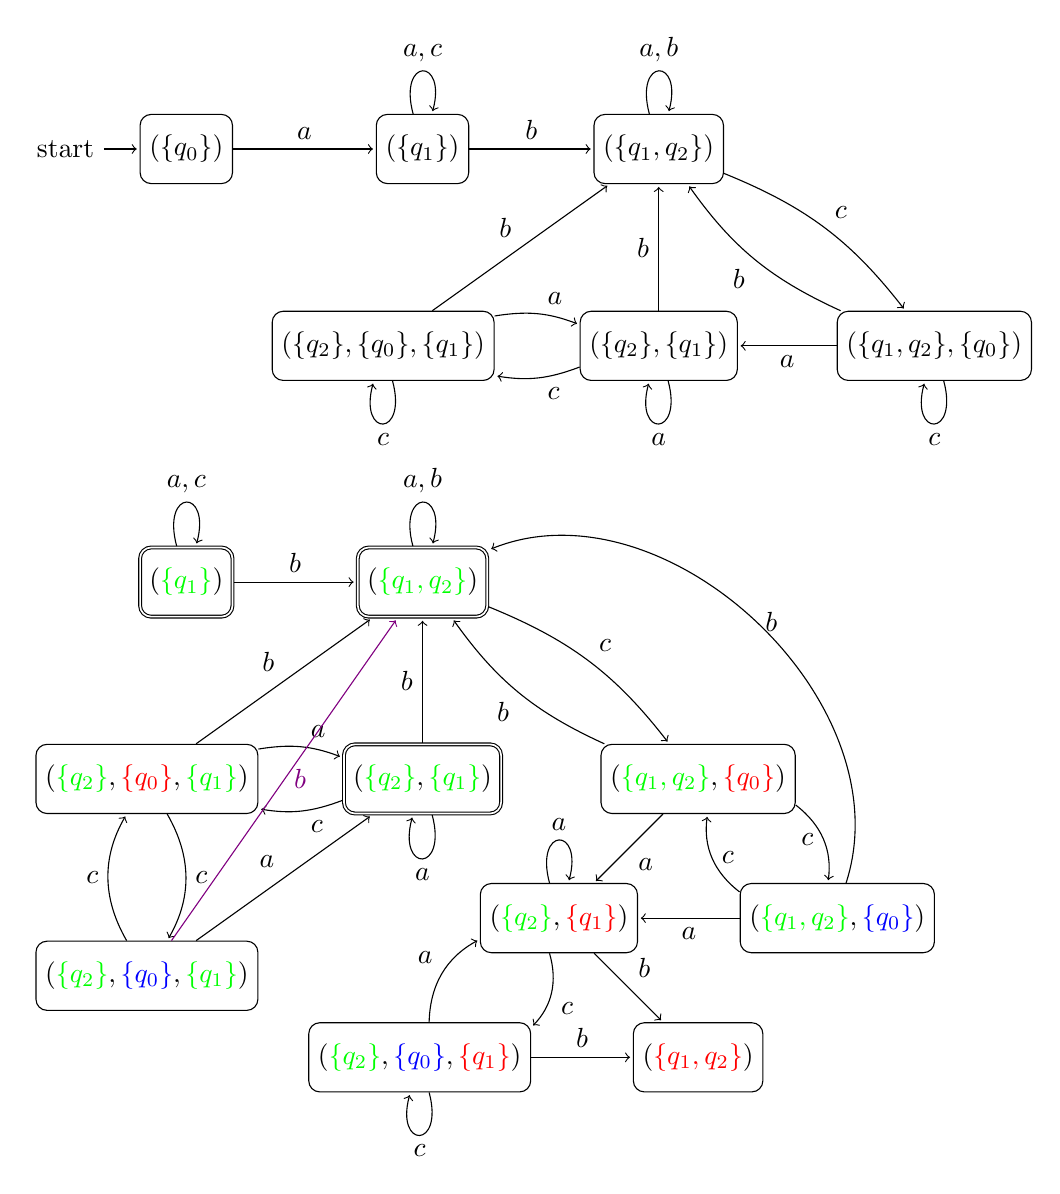
\begin{tikzpicture}[shorten >=1pt,node distance=2.5cm,on grid,auto]
      
      \tikzset{rounded/.style={draw,rectangle,rounded corners}}
      \node[state,rounded,initial] (q0) {$(\{q_0\})$};
      \node[state,rounded] (q1) [right = 3cm of q0] {$(\{q_1\})$};
      \node[state,rounded] (q1q2) [right = 3cm of q1] {$(\{q_1,q_2\})$};
      \node[state,rounded] (q2q1)   [below = of q1q2] {$(\{q_2\},\{q_1\})$};
      \node[state,rounded] (q1q2q0) [right = 3.5cm of q2q1] {$(\{q_1,q_2\},\{q_0\})$};
      \node[state,rounded] (q2q0q1) [left = 3.5cm of q2q1] {$(\{q_2\},\{q_0\},\{q_1\})$};

      \node[state,rounded,accepting] (q1b) [below = 5.5cm of q0] {$(\textcolor{green}{\{q_1\}})$};
      \node[state,rounded,accepting] (q1q2b) [right = 3cm of q1b] {$(\textcolor{green}{\{q_1,q_2\}})$};
      \node[state,rounded,accepting] (q2q1b)   [below = of q1q2b] {$(\textcolor{green}{\{q_2\}},\textcolor{green}{\{q_1\}})$};
      \node[state,rounded] (q1q2q0b) [right = 3.5cm of q2q1b] {$(\textcolor{green}{\{q_1,q_2\}},\textcolor{red}{\{q_0\}})$};
      \node[state,rounded] (q2q0q1b) [left = 3.5cm of q2q1b] {$(\textcolor{green}{\{q_2\}},\textcolor{red}{\{q_0\}},\textcolor{green}{\{q_1\}})$};

      
      \node[state,rounded] (q2q1c)   [below left = of q1q2q0b] {$(\textcolor{green}{\{q_2\}},\textcolor{red}{\{q_1\}})$};
      \node[state,rounded] (q1q2q0c) [below right = of q1q2q0b] {$(\textcolor{green}{\{q_1,q_2\}},\textcolor{blue}{\{q_0\}})$};
      \node[state,rounded] (q1q2c) [below right = of q2q1c] {$(\textcolor{red}{\{q_1,q_2\}})$};
      
      \node[state,rounded] (q2q0q1c) [below left = of q2q1c] {$(\textcolor{green}{\{q_2\}},\textcolor{blue}{\{q_0\}},\textcolor{red}{\{q_1\}})$};
      \node[state,rounded] (q2q0q1d) [below = of q2q0q1b] {$(\textcolor{green}{\{q_2\}},\textcolor{blue}{\{q_0\}},\textcolor{green}{\{q_1\}})$};

      \path[->]
      (q0)
      edge [] node [] {$a$} (q1)
      (q1)
      edge [loop above] node [] {$a,c$} ()
      edge [] node [] {$b$} (q1q2)
      (q1q2)
      edge [loop above] node [] {$a,b$} ()
      edge [bend left = 15] node [] {$c$} (q1q2q0)
      (q2q1)
      edge [loop below] node [] {$a$} ()
      edge [] node [] {$b$} (q1q2)
      edge [bend left = 15] node [] {$c$} (q2q0q1)
      (q1q2q0)
      edge [] node [] {$a$} (q2q1)
      edge [bend left = 15] node [] {$b$} (q1q2)
      edge [loop below] node [] {$c$} ()
      (q2q0q1)
      edge [bend left = 15] node [] {$a$} (q2q1)
      edge [] node [] {$b$} (q1q2)
      edge [loop below] node [] {$c$} ()
      (q1b)
      edge [loop above] node [] {$a,c$} ()
      edge [] node [] {$b$} (q1q2b)
      (q1q2b)
      edge [loop above] node [] {$a,b$} ()
      edge [bend left = 15] node [] {$c$} (q1q2q0b)
      (q1q2q0b)
      edge [] node [] {$a$} (q2q1c)
      edge [bend left = 15] node [] {$b$} (q1q2b)
      edge [bend left] node [left] {$c$} (q1q2q0c)
      (q1q2q0c)
      edge [] node [] {$a$} (q2q1c)
      edge [bend right = 65] node [right] {$b$} (q1q2b)
      edge [bend left] node [right] {$c$} (q1q2q0b)
      (q2q1c)
      edge [loop above] node [] {$a$} ()
      edge [] node [] {$b$} (q1q2c)
      edge [bend left] node [] {$c$} (q2q0q1c)
      (q2q0q1c)
      edge [bend left] node [] {$a$} (q2q1c)
      edge [] node [] {$b$} (q1q2c)
      edge [loop below] node [] {$c$} ()
      (q2q1b)
      edge [loop below] node [] {$a$} ()
      edge [] node [] {$b$} (q1q2b)
      edge [bend left = 15] node [] {$c$} (q2q0q1b)
      (q2q0q1b)
      edge [bend left = 15] node [] {$a$} (q2q1b)
      edge [] node [] {$b$} (q1q2b)
      edge [bend left] node [] {$c$} (q2q0q1d)
      (q2q0q1d)
      edge [] node [] {$a$} (q2q1b)
      edge [violet] node [right] {$b$} (q1q2b)
      edge [bend left] node [] {$c$} (q2q0q1b)
      ;
    \end{tikzpicture}
  \end{turn}
}

\newpage

\section*{Runs}

We use the followig automaton for the runs (to simplify the reading and
writing...) :
\begin{center}
  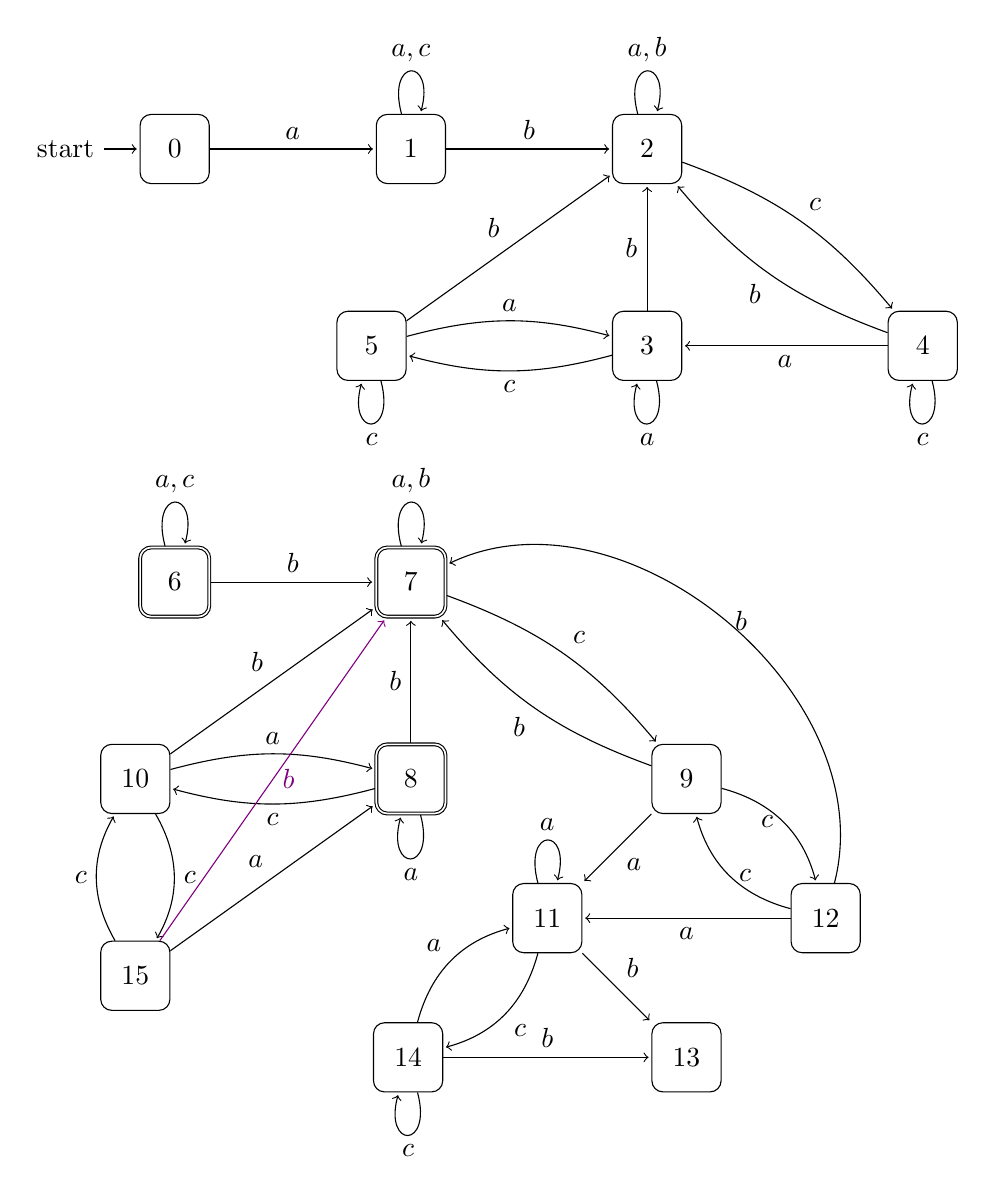
\begin{tikzpicture}[shorten >=1pt,node distance=2.5cm,on grid,auto]
    
    \tikzset{rounded/.style={draw,rectangle,rounded corners}}
    \node[state,rounded,initial] (q0) {$0$};
    \node[state,rounded] (q1) [right = 3cm of q0] {$1$};
    \node[state,rounded] (q1q2) [right = 3cm of q1] {$2$};
    \node[state,rounded] (q2q1)   [below = of q1q2] {$3$};
    \node[state,rounded] (q1q2q0) [right = 3.5cm of q2q1] {$4$};
    \node[state,rounded] (q2q0q1) [left = 3.5cm of q2q1] {$5$};
    \node[state,rounded,accepting] (q1b) [below = 5.5cm of q0] {$6$};
    \node[state,rounded,accepting] (q1q2b) [right = 3cm of q1b] {$7$};
    \node[state,rounded,accepting] (q2q1b)   [below = of q1q2b] {$8$};
    \node[state,rounded] (q1q2q0b) [right = 3.5cm of q2q1b] {$9$};
    \node[state,rounded] (q2q0q1b) [left = 3.5cm of q2q1b] {$10$};
    \node[state,rounded] (q2q1c)   [below left = of q1q2q0b] {$11$};
    \node[state,rounded] (q1q2q0c) [below right = of q1q2q0b] {$12$};
    \node[state,rounded] (q1q2c) [below right = of q2q1c] {$13$};
    \node[state,rounded] (q2q0q1c) [below left = of q2q1c] {$14$};
    \node[state,rounded] (q2q0q1d) [below = of q2q0q1b] {$15$};

    \path[->]
    (q0)
    edge [] node [] {$a$} (q1)
    (q1)
    edge [loop above] node [] {$a,c$} ()
    edge [] node [] {$b$} (q1q2)
    (q1q2)
    edge [loop above] node [] {$a,b$} ()
    edge [bend left = 15] node [] {$c$} (q1q2q0)
    (q2q1)
    edge [loop below] node [] {$a$} ()
    edge [] node [] {$b$} (q1q2)
    edge [bend left = 15] node [] {$c$} (q2q0q1)
    (q1q2q0)
    edge [] node [] {$a$} (q2q1)
    edge [bend left = 15] node [] {$b$} (q1q2)
    edge [loop below] node [] {$c$} ()
    (q2q0q1)
    edge [bend left = 15] node [] {$a$} (q2q1)
    edge [] node [] {$b$} (q1q2)
    edge [loop below] node [] {$c$} ()
    (q1b)
    edge [loop above] node [] {$a,c$} ()
    edge [] node [] {$b$} (q1q2b)
    (q1q2b)
    edge [loop above] node [] {$a,b$} ()
    edge [bend left = 15] node [] {$c$} (q1q2q0b)
    (q1q2q0b)
    edge [] node [] {$a$} (q2q1c)
    edge [bend left = 15] node [] {$b$} (q1q2b)
    edge [bend left] node [left] {$c$} (q1q2q0c)
    (q1q2q0c)
    edge [] node [] {$a$} (q2q1c)
    edge [bend right = 65] node [right] {$b$} (q1q2b)
    edge [bend left] node [right] {$c$} (q1q2q0b)
    (q2q1c)
    edge [loop above] node [] {$a$} ()
    edge [] node [] {$b$} (q1q2c)
    edge [bend left] node [] {$c$} (q2q0q1c)
    (q2q0q1c)
    edge [bend left] node [] {$a$} (q2q1c)
    edge [] node [] {$b$} (q1q2c)
    edge [loop below] node [] {$c$} ()
    (q2q1b)
    edge [loop below] node [] {$a$} ()
    edge [] node [] {$b$} (q1q2b)
    edge [bend left = 15] node [] {$c$} (q2q0q1b)
    (q2q0q1b)
    edge [bend left = 15] node [] {$a$} (q2q1b)
    edge [] node [] {$b$} (q1q2b)
    edge [bend left] node [] {$c$} (q2q0q1d)
    (q2q0q1d)
    edge [] node [] {$a$} (q2q1b)
    edge [violet] node [right] {$b$} (q1q2b)
    edge [bend left] node [] {$c$} (q2q0q1b)
    ;
  \end{tikzpicture}
\end{center}

\subsection*{Run for $(aabbcc)^\omega$}

$(aabbcc)^\omega$ is accepted by the original automaton : $012220\ 012220\
012220 \dots$ so it should not be accepted by its complement.

\subsubsection*{Run 1}
\[
  0\ 6\ 6\ 7\ 7\ 9\ 12\ 11\ 11\ 13\dots
\]

From the state $13$, we can't accept any words since all of its components are red.


\subsubsection*{Run 2}
\[
  0\ 1\ 1\ 2\ 2\ 4\ 9\ 12\ 11\ 11\ 13\dots
\]

\subsection*{Run for $(abcb)^\omega$}

$(aabbcc)^\omega$ is not accepted by the original automaton. So its complement
should accept it.

\subsubsection*{Run 1}
\[
  0\ 6\ 7\ 9\ 7\ 7\ 7\ 9\ 7\ 7\ 7\ 9\ 7\ 7\ 7\ \dots
\]

\subsubsection*{Run 2}
\[
  0\ 1\ 2\ 4\ 2\ 2\ 2\ 4\ 2\ 2\ 2\ (\dots) 4\ 2\ 2\ 2\ 9\ 7\ 7\ 7\  9\ 7\ 7\ 7\ \dots
\]

Both of those runs are accepting.

\end{document}